\section{Evaluation}
\label{eval}

\subsection{YFCC100M Dataset}
\label{dataset}

Here goes an explanation of the dataset and all the source
(images, metadata, videos, features).

\subsection{Experimental Setup}

Here goes explanation of the comparison systems.
Need versions of MYSQL, OS, amount of memory and CPU info.

\begin{figure*}[]
\centering
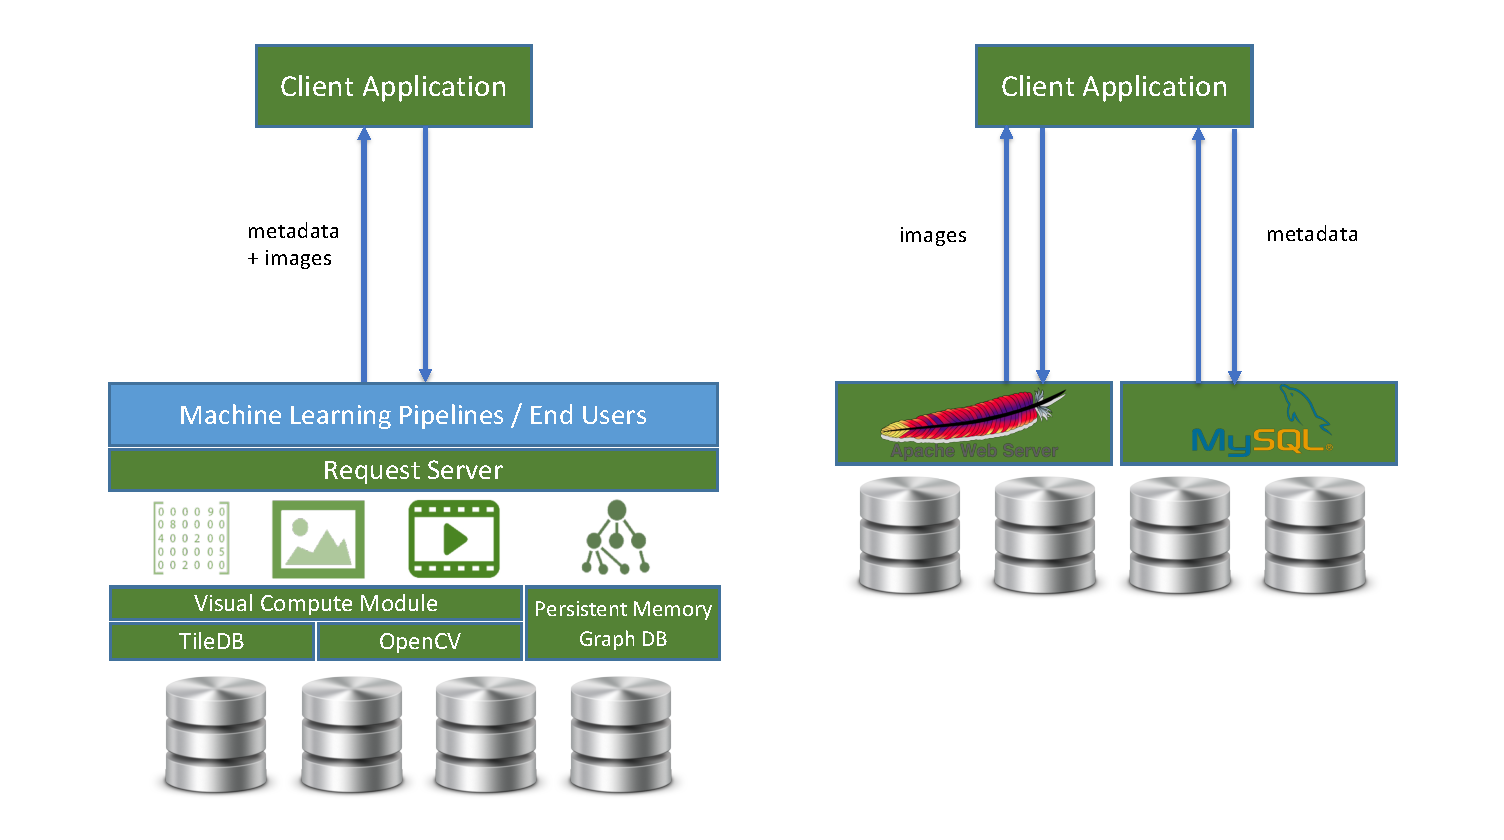
\includegraphics[width=\textwidth]{figures/comparison_system}
\caption{Comparison Systems}
\label{fig:systems}
\end{figure*}

\subsection{Images + Metadata}

Explanation of the evaluation and description of some of the queries.

\begin{figure}[]
\centering
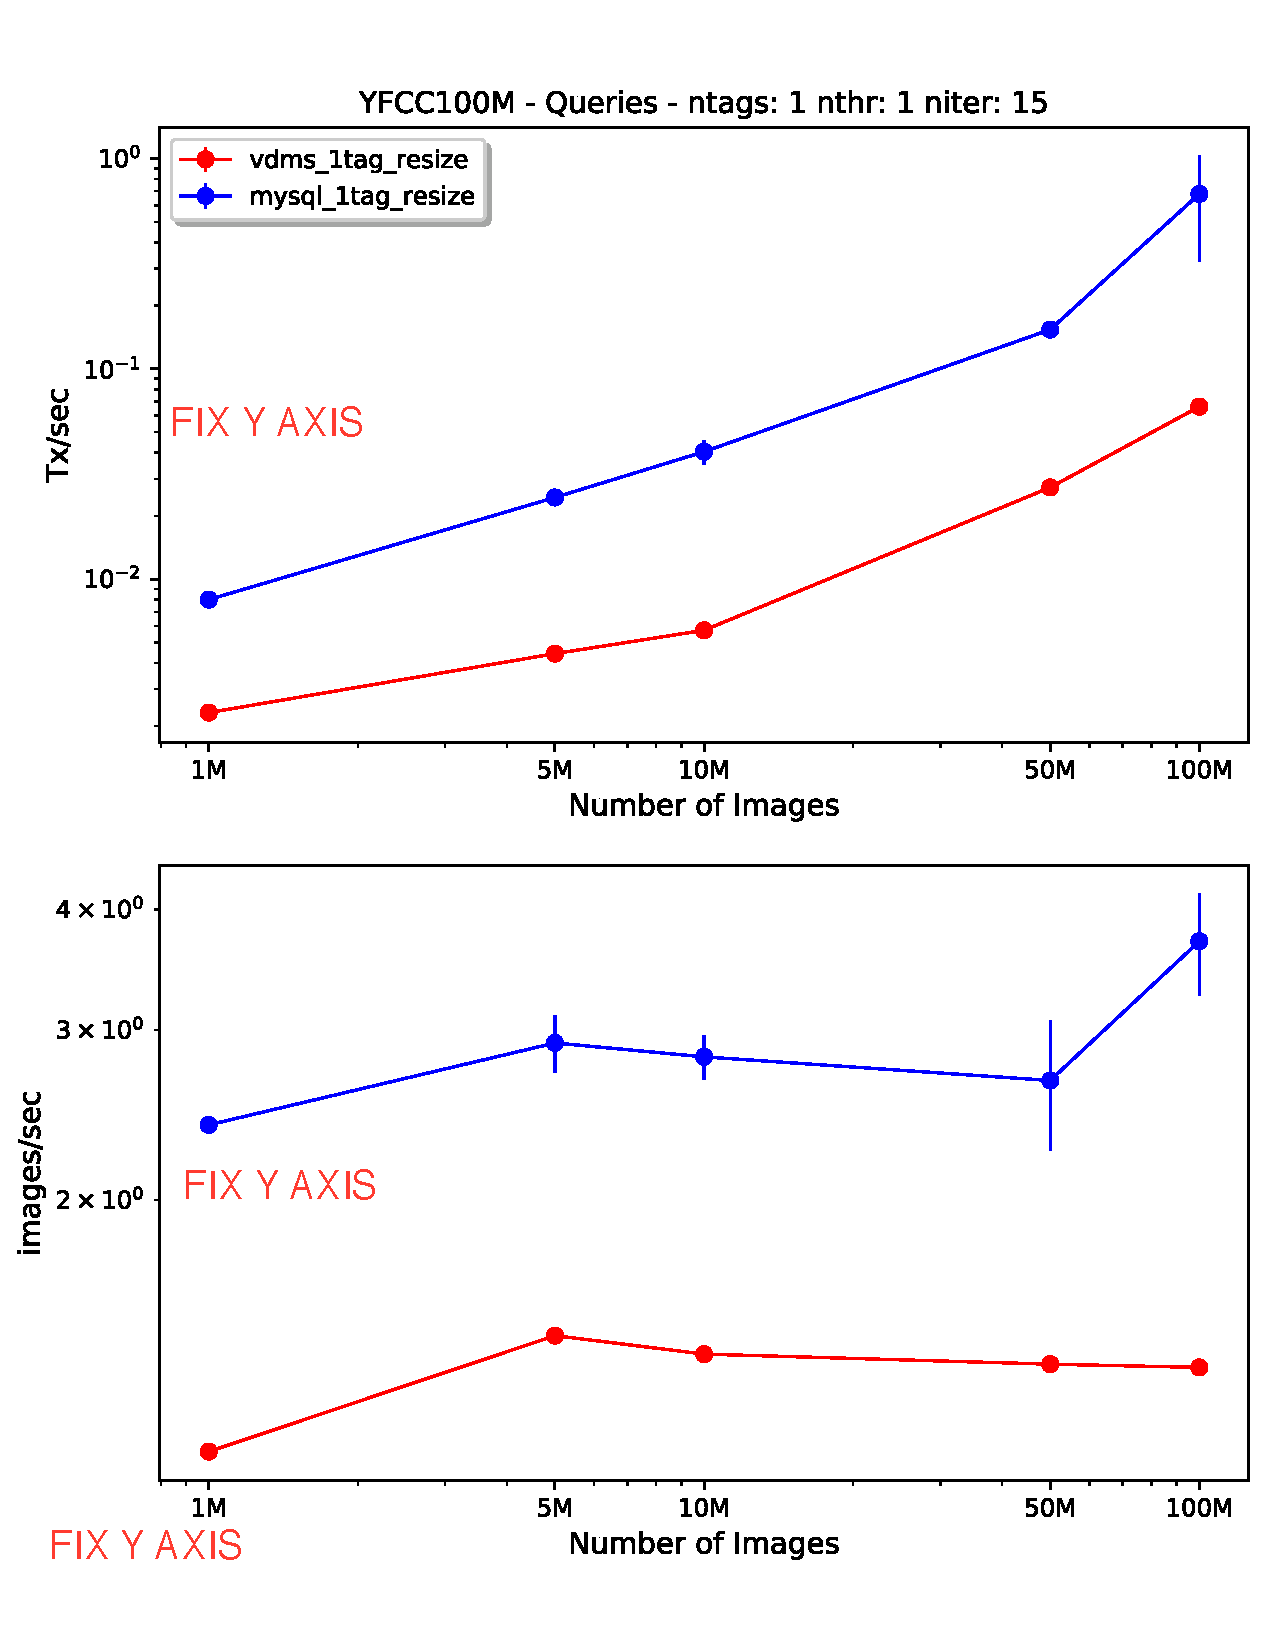
\includegraphics[width=\columnwidth]{figures/q1_latency}
\caption{Query 1 - Latency}
\label{fig:q1_latency}
\end{figure}

\begin{figure}[]
\centering
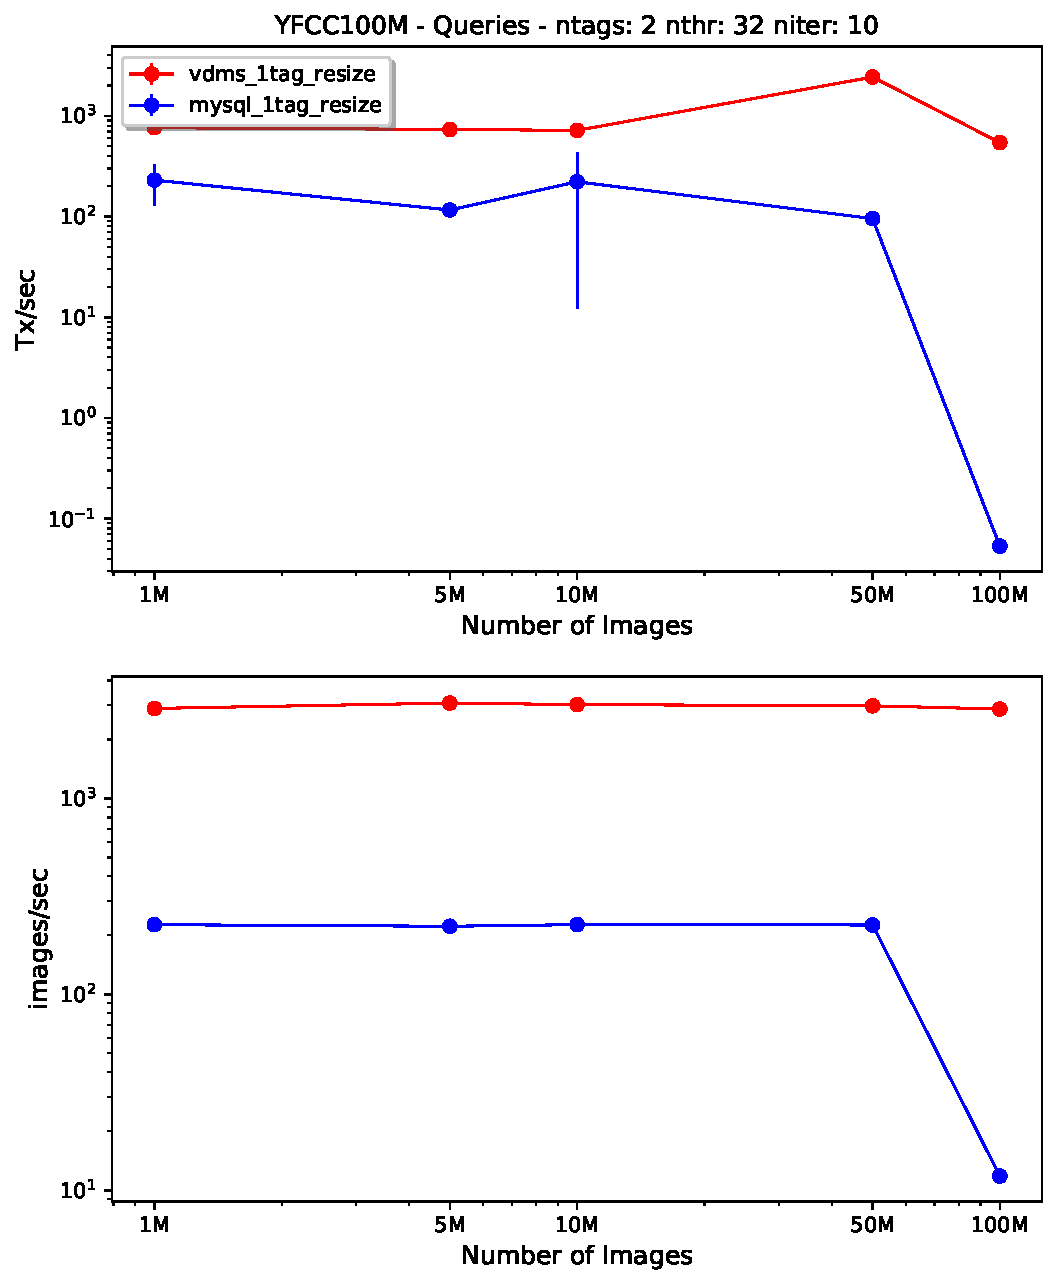
\includegraphics[width=\columnwidth]{figures/q1_throughput}
\caption{Query 1 - Throughput}
\label{fig:q1_throughput}
\end{figure}

\subsection{Videos}

Explanation of the video queries and comparison.
Explain concurrency.

\begin{figure*}[]
\centering
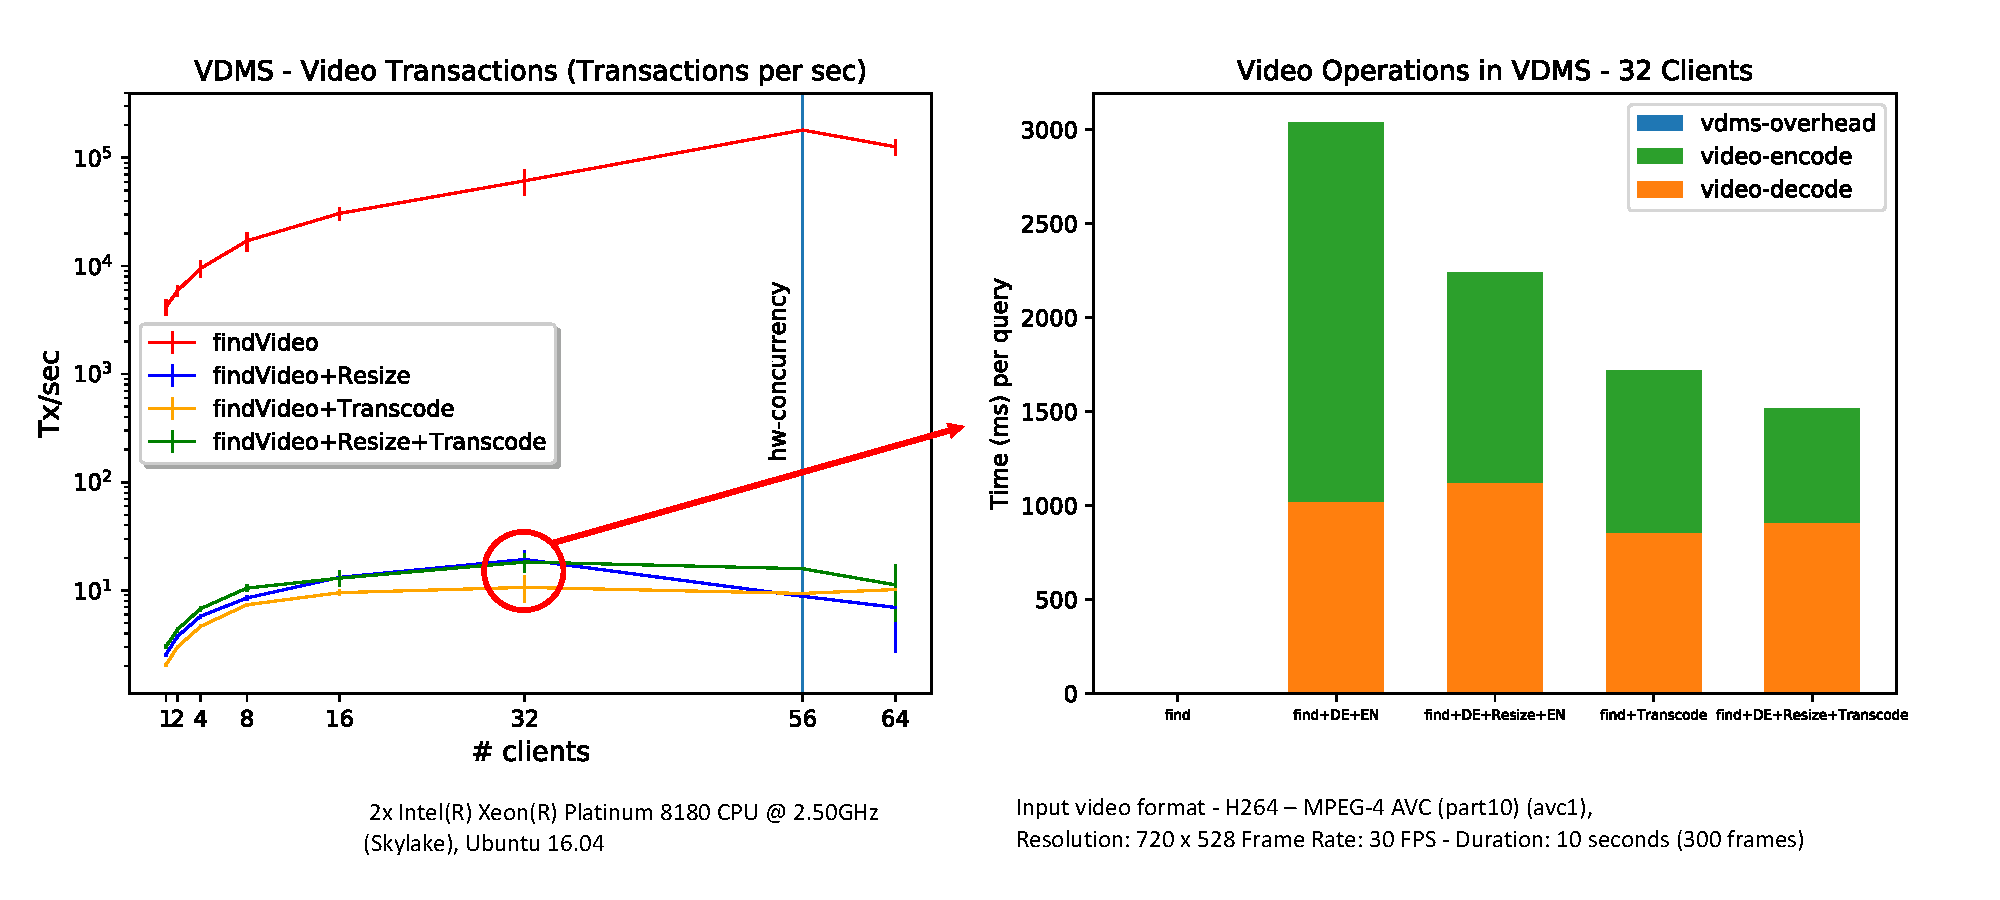
\includegraphics[width=\textwidth]{figures/video_overhead}
\caption{Concurrency and Overhead}
\label{fig:video}
\end{figure*}

\subsection{Feature Vectors}

Explain different engines supported, and how the features vectors
were ingested and handled.

\begin{figure*}[]
\centering
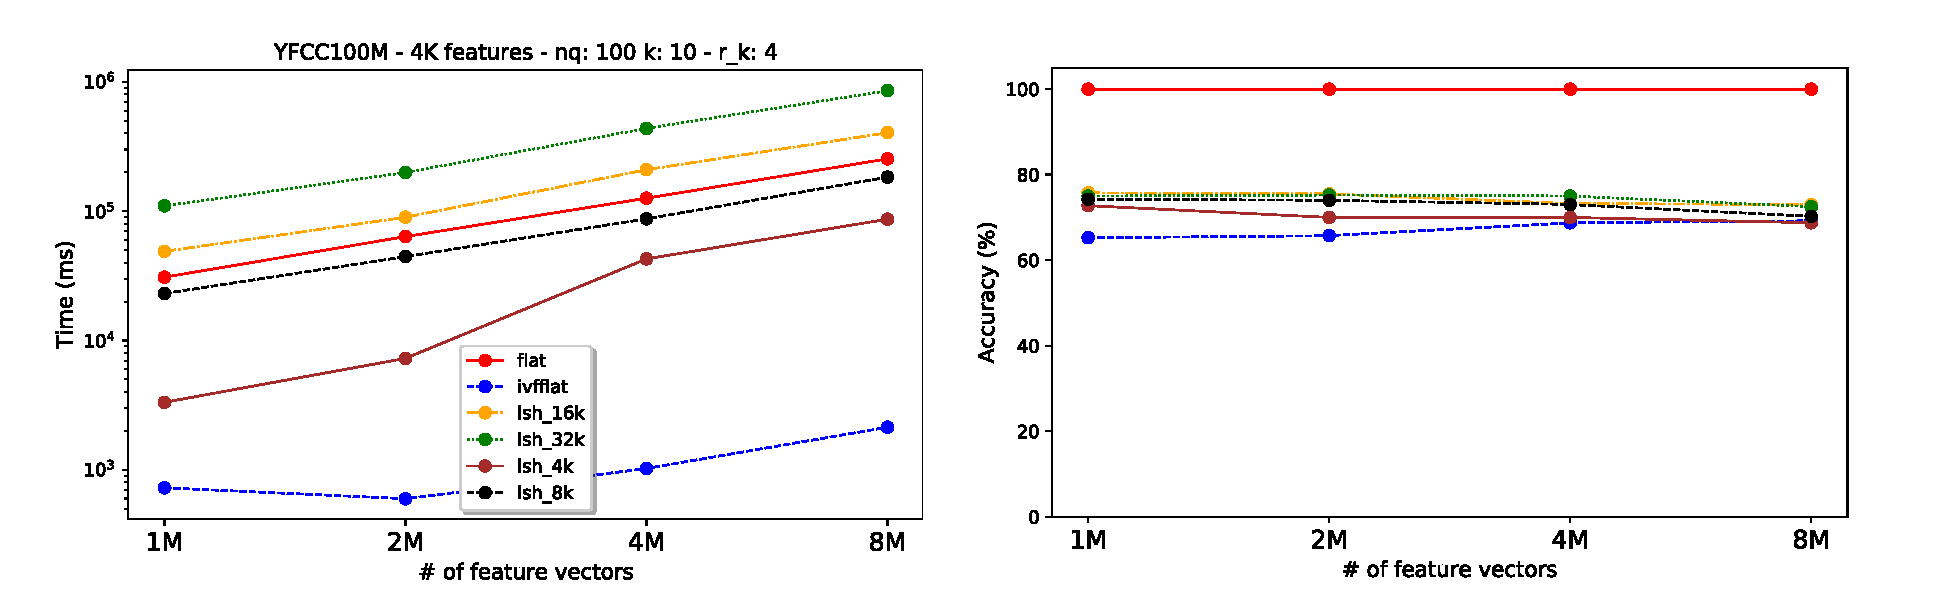
\includegraphics[width=\textwidth]{figures/features_alternatives}
\caption{Feature Vector Evaluation}
\label{fig:features_eval}
\end{figure*}

\begin{figure*}[]
\centering
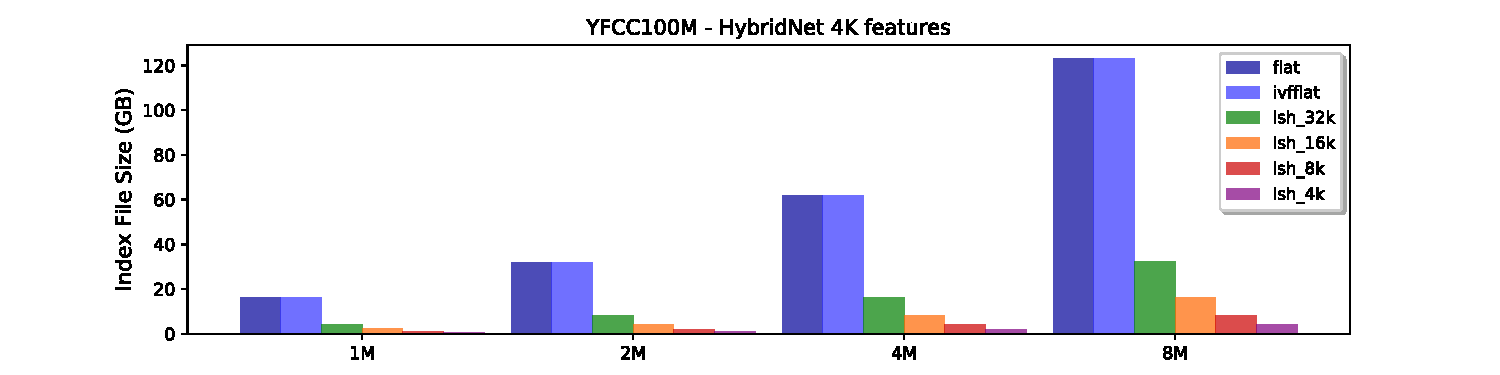
\includegraphics[width=\textwidth]{figures/features_disksize}
\caption{Feature Collection Size in Disk}
\label{fig:features_size_does_matter}
\end{figure*}
